\documentclass[dvipsnames,11pt]{article}
\usepackage{amsmath}

%Hey, if you're using this preamble it means that it was probably written by Stefano Graziosi (me). If you see something that doesn't make sense, feel free to email me at stefano.graziosi@studbocconi.it
%p.s. in case it's not already evident from the preamble, I'm not a professional LaTeX user, so I'm sure there are better ways to do things. I'm just trying to make it work.

%------------------------------------------------------------------------------
%           LAST UPDATE: 30-01-2025
%------------------------------------------------------------------------------

%I don't own copyright on anything, I just literally copied and pasted together a bunch of stuff.

%Credit goes to the original authors.

%------------------------------------------------------------------------------
%           Packages
%------------------------------------------------------------------------------

\usepackage{fancyhdr}
\usepackage[dvipsnames]{xcolor}
\usepackage[many]{tcolorbox}
\usepackage[all]{xy}
\usepackage{tcolorbox}
\usepackage{graphicx}
\usepackage{hyperref}
\usepackage{xcolor}    
\usepackage{wrapfig}
\usepackage{amsmath, amssymb, amsthm}
\usepackage{titlesec}
\usepackage{halloweenmath}
\usepackage{enumitem}
\usepackage{listings}
\usepackage{kantlipsum}
\usepackage{pdfpages}

\usepackage[T1]{fontenc}                            % Font Styling
\usepackage{lmodern,mathrsfs}


\usepackage{mathtools,amsthm,amssymb,amsfonts,bm}   % Math Presets
\usepackage{thmtools,amsmath}
\usepackage{array,tabularx,booktabs}                % Table Presets
\usepackage{graphicx,wrapfig,float,caption}         % Figure Presets
\usepackage{setspace,multicol}                      % Text Presets
\usepackage{tikz,physics}                           % Physics Presets

\usepackage{titlepic}
\usepackage{pdfpages}

%------------------------------------------------------------------------------
%           Geometry
%------------------------------------------------------------------------------

\usepackage[a4paper,margin=1in]{geometry}
%\usepackage[margin=1in]{geometry}

%------------------------------------------------------------------------------
%           Chapter and section formatting
%------------------------------------------------------------------------------

%\renewcommand{\chaptername}{Lecture}
%\renewcommand\thesection{P~\arabic{section}}

\renewcommand{\thefigure}{\thesection-\arabic{figure}}
\renewcommand{\thetable}{\thesection-\arabic{table}}

%------------------------------------------------------------------------------
%           Colours
%------------------------------------------------------------------------------

\definecolor{sgblue}{rgb}{0, 169, 211}
\definecolor{sggreen}{rgb}{0, 164, 0}
\definecolor{sgpurple}{rgb}{99, 0, 165}
\definecolor{sgyellow}{rgb}{255, 211, 0}
\definecolor{sgorange}{rgb}{255, 127, 20}

\definecolor{sbblue}{rgb}{219, 248, 254}
\definecolor{sbgreen}{rgb}{223, 255, 218}
\definecolor{sbpurple}{rgb}{241, 220, 255}

\definecolor{codegreen}{rgb}{0,0.6,0}
\definecolor{codegray}{rgb}{0.5,0.5,0.5}
\definecolor{codepurple}{rgb}{0.58,0,0.82}
\definecolor{backcolour}{rgb}{0.95,0.95,0.92}

%------------------------------------------------------------------------------
%           Environments
%------------------------------------------------------------------------------

%Standard \latex box

\newtcolorbox{mybox}[3][]
{
  colframe = #2!25,
  colback  = #2!10,
  coltitle = #2!20!black,  
  title    = {#3},
  #1,
}

%Standard "Problem" environment

\newtheorem{problem}{Problem}

%Personalised "Solution" environment

\newenvironment{solution}[1][\it{\textcolor{MidnightBlue}{Solution}}]{\textbf{#1. } }{\textcolor{MidnightBlue}{$\square$}}


% ----------------------------------------------------------------------
%           Special Environments 
% ----------------------------------------------------------------------

\newlength{\spacelength}
\settowidth{\spacelength}{\normalfont\ }
\declaretheoremstyle[
    headfont={\bfseries\sffamily\footnotesize},
    notefont={\normalfont},
    bodyfont={\normalfont},
    headpunct={\relax},%\newline,
    headformat={%
        \makebox[0pt][r]{\NAME\ \NUMBER\hspace{\marginparsep}}\hskip-\spacelength{\normalsize\NOTE}},
]{theorem}

\tcolorboxenvironment{theorem}{
  boxrule=0pt,
  boxsep=0pt,
  colback={White},
  enhanced jigsaw, 
  borderline west={1pt}{0pt}{ForestGreen},
  sharp corners,
  before skip=10pt,
  after skip=10pt,
  left=5pt,
  right=5pt,
  breakable,
}

\declaretheorem[style=theorem]{proposition}

\let\proof\relax
\let\endproof\relax

\declaretheoremstyle[
    headfont={\bfseries\sffamily\footnotesize},
    notefont={\normalfont},
    bodyfont={\normalfont},
    headpunct={\relax},%\newline,
    headformat={%
        \makebox[0pt][r]{\NAME\ \NUMBER\hspace{\marginparsep}}\hskip-\spacelength{\normalsize\NOTE}},
]{theorem}

\tcolorboxenvironment{proposition}{
  boxrule=0pt,
  boxsep=0pt,
  colback={White},
  enhanced jigsaw, 
  borderline west={1pt}{0pt}{Mulberry},
  sharp corners,
  before skip=10pt,
  after skip=10pt,
  left=5pt,
  right=5pt,
  breakable,
}

\declaretheorem[style=theorem]{theorem}

\let\proof\relax
\let\endproof\relax

\declaretheoremstyle[
    headfont={\small\scshape},
    notefont={\normalfont},
    bodyfont={\normalfont},
    headpunct={\relax},
    headformat={%
        \makebox[0pt][r]{\NAME\hspace{\marginparsep}}\hskip-\spacelength{\NOTE}},
]{proof}

\tcolorboxenvironment{proof}{
  boxrule=0pt,
  boxsep=0pt,
  blanker,
  borderline west={1pt}{0pt}{black},
  before skip=10pt,
  after skip=10pt,
  left=5pt,
  right=5pt,
  breakable,
}

\declaretheoremstyle[
    headfont={\footnotesize\itshape},
    notefont={\normalfont},
    bodyfont={\normalfont},
    headpunct={\relax},
    headformat={%
        \makebox[0pt][r]{\NAME\hspace{\marginparsep}}\hskip-\spacelength{\NOTE}},
]{claim}

\declaretheorem[
    style=proof,
    qed=\qedsymbol]{proof}

\declaretheorem[style=claim]{Intuition}

\theoremstyle{theorem}
\newtheorem{ques}{Question}

\theoremstyle{theorem}
\newtheorem{definition}{Definition}
\tcolorboxenvironment{definition}{
  boxrule=0pt,
  boxsep=0pt,
  colback={White},
  enhanced jigsaw, 
  borderline west={1pt}{0pt}{Cerulean},
  sharp corners,
  before skip=10pt,
  after skip=10pt,
  left=5pt,
  right=5pt,
  breakable,
}

\theoremstyle{theorem}
\newtheorem{lemma}{Lemma}
\tcolorboxenvironment{lemma}{
  boxrule=0pt,
  boxsep=0pt,
  blanker,
  borderline west={1pt}{0pt}{Rhodamine},
  before skip=10pt,
  after skip=10pt,
  sharp corners,
  left=5pt,
  right=5pt,
  breakable,
}

\theoremstyle{theorem}
\newtheorem{remark}{Remark}
\tcolorboxenvironment{remark}{
  boxrule=0pt,
  boxsep=0pt,
  colback={White},
  enhanced jigsaw, 
  borderline west={1pt}{0pt}{BurntOrange},
  before skip=10pt,
  after skip=10pt,
  sharp corners,
  left=5pt,
  right=5pt,
  breakable,
}

\theoremstyle{theorem}
\newtheorem{corollary}{Corollary}
\tcolorboxenvironment{corollary}{
  boxrule=0pt,
  boxsep=0pt,
%  colback={White!100!WildStrawberry},
  enhanced jigsaw,
  borderline west={1pt}{0pt}{WildStrawberry},
  before skip=10pt,
  after skip=10pt,
  sharp corners,
  left=5pt,
  right=5pt,
  breakable,
}

\theoremstyle{theorem}
\newtheorem{example}{Example}
\tcolorboxenvironment{example}{
  boxrule=0pt,
  boxsep=0pt,
  blanker,
  borderline west={1pt}{0pt}{Dandelion},
  before skip=10pt,
  after skip=10pt,
  sharp corners,
  left=5pt,
  right=5pt,
  breakable,
}


\theoremstyle{claim}
\newtheorem{intu}{Intuition}

\theoremstyle{claim}
\newtheorem{solu}{Solution}

%------------------------------------------------------------------------------
%           Code Listing Environment
%------------------------------------------------------------------------------

\lstdefinestyle{mystyle}{
    backgroundcolor=\color{backcolour},   
    commentstyle=\color{codegreen},
    keywordstyle=\color{magenta},
    numberstyle=\tiny\color{codegray},
    stringstyle=\color{codepurple},
    basicstyle=\ttfamily\footnotesize,
    breakatwhitespace=false,         
    breaklines=true,                 
    captionpos=b,                    
    keepspaces=true,                 
    numbers=left,                    
    numbersep=5pt,                  
    showspaces=false,                
    showstringspaces=false,
    showtabs=false,                  
    tabsize=2
}

\lstset{style=mystyle}

\setlength{\headheight}{25pt} % Non so perché ma senza questo da un piccolo errore

\pagestyle{fancy}
\fancyhf{} 
\fancyhead[L]{\textsc{\footnotesize{PhD in Economics and Finance} \\ \small{40313 Introd. to Probability}}} 
\fancyhead[R]{\textsc{\small Graziosi \\ Natalucci}} 
\fancyhead[C]{\textbf{Problem set 5}}
\fancyfoot[C]{\thepage} 
\renewcommand{\headrulewidth}{0.4pt} 
\renewcommand{\footrulewidth}{0pt}

\usetikzlibrary{arrows.meta}

\tikzset{
  state/.style={circle, minimum size=10mm, shading=ball, ball color=blue!25,
                draw=black, thick, text=black},
  prob/.style={midway, sloped, fill=white, inner sep=1pt, font=\small}
}

\begin{document}

\setcounter{section}{1}
\section*{Question 1}

\textbf{1.} Let $X_n$ be a Markov chain with state space $S=\{1,2,3\}$ and transition matrix
\[
\mathbf{P}=\left[
\begin{array}{ccc}
0 &1/2 &1/2\\
1/ 2 &0 &1/ 2\\
1/ 2 &1/ 2& 0
\end{array}
\right].
\]

\begin{figure}[ht]
    \centering
        \begin{tikzpicture}[>=Latex]
        
        % --- States (as balls at triangle vertices)
        \node[state] (1) at (0,0) {1};
        \node[state] (2) at (4,0) {2};
        \node[state] (3) at (2,3.2) {3};
        
        % --- Transitions 1 <-> 2
        \draw[->, bend left=18] (1) to node[prob, above] {$\tfrac{1}{2}$} (2);
        \draw[->, bend left=18] (2) to node[prob, above] {$\tfrac{1}{2}$} (1);
        
        % --- Transitions 1 <-> 3
        \draw[->, bend left=18] (1) to node[prob, above] {$\tfrac{1}{2}$} (3);
        \draw[->, bend left=18] (3) to node[prob, above] {$\tfrac{1}{2}$} (1);
        
        % --- Transitions 2 <-> 3
        \draw[->, bend left=18] (2) to node[prob, above] {$\tfrac{1}{2}$} (3);
        \draw[->, bend left=18] (3) to node[prob, above] {$\tfrac{1}{2}$} (2);
        
        \end{tikzpicture}
    \caption{Visual repreesntation of the Markov chain}
    \label{fig:placeholder}
\end{figure}

    \begin{enumerate}[label=\alph*.]
        \item Find the 2-step transition probabilities.
    
            \begin{solution}
    
                By definition, $\mathbf{P}^{(2)}=\mathbf{P}^2$. For $i=j$,
                \[
                p^{(2)}_{ii}=\sum_{k}p_{ik}p_{ki}
                = p_{ij}p_{ji}+p_{i\ell}p_{\ell i}
                = \tfrac12\cdot\tfrac12+\tfrac12\cdot\tfrac12=\tfrac12,
                \]
                where $\{j,\ell\}=S\setminus\{i\}$. For $i\neq j$,
                \[
                p^{(2)}_{ij}=\sum_{k}p_{ik}p_{kj}
                = p_{ii}p_{ij}+p_{ij}p_{jj}+p_{i\ell}p_{\ell j}
                = 0 + 0 + \tfrac12\cdot\tfrac12=\tfrac14.
                \]
                Hence
                \[
                \mathbf{P}^2=\begin{bmatrix}
                \tfrac12 & \tfrac14 & \tfrac14\\
                \tfrac14 & \tfrac12 & \tfrac14\\
                \tfrac14 & \tfrac14 & \tfrac12
                \end{bmatrix}.
                \]
                
            \end{solution}
            
        \item Is the chain periodic?
    
            \begin{solution}
    
                The period of state $i$ is $\gcd\{n\ge 1: p^{(n)}_{ii}>0\}$ (Ch. 4.5.1). Since $p^{(2)}_{11}>0$ and also $p^{(3)}_{11}>0$ (e.g., $1\to 2\to 3\to 1$ has positive probability), the set of return times contains $2$ and $3$, so $\gcd(2,3)=1$. Thus state $1$ has period $1$; by irreducibility (which we discuss more in detail in the next subquestion) all states share the same period, so the chain is \emph{aperiodic}.
                
            \end{solution}
            
        \item Is the chain irreducible?
    
            \begin{solution}
    
                Yes. From each state we can reach any other state in one step (all off-diagonal entries of $\mathbf{P}$ are positive), so all states communicate; by the definition the chain is irreducible.
                
            \end{solution}

        \item Find the stationary distribution.

            \begin{solution}

                A stationary distribution $\pi$ satisfies $\pi P=\pi$ and $\sum_i\pi_i=1$. Here $P$ is doubly stochastic (row and column sums are $1$), hence the uniform vector is stationary:
                \[
                \pi=\left(\tfrac13,\tfrac13,\tfrac13\right).
                \]
                We can check this directly by observing that:
                \begin{align}
                    \pi \mathbf{P} &=\pi \\
                    \left(\frac{1}{3},\frac{1}{3},\frac{1}{3}\right) \times \left[
                    \begin{array}{ccc}
                    0 & \tfrac12 & \tfrac12 \\
                    \tfrac12 & 0 & \tfrac12 \\
                    \tfrac12 & \tfrac12 & 0
                    \end{array}
                    \right] & = \left(\frac{1}{3},\frac{1}{3},\frac{1}{3}\right)
                \end{align}
                
            \end{solution}
            
        \item If the chain starts in 1, is the chain stationary?
    
            \begin{solution}
    
                No. “Stationary” for a time-homogeneous Markov chain means the initial law is a stationary distribution (so all marginal laws are constant over time). Starting in $1$ means the initial distribution is $\delta_1\neq \pi$, hence the process is \emph{not} stationary.
                
            \end{solution}
            
        \item Find $\lim_{n\rightarrow\infty}\mathbf{P}(X_n= 1)$ if the chain starts in 1.
    
            \begin{solution}

                For finite, irreducible, aperiodic Markov chains, $\mathbf{P}^n(i,\cdot)\to\pi(\cdot)$ as $n\to\infty$ (convergence to the unique stationary distribution). Thus
                \[
                \lim_{n\to\infty}\mathbf P(X_n=1\mid X_0=1)=\pi_1=\tfrac13.
                \]
                
            \end{solution}
            
        \item Would the answer to point f. change if the initial probabilities were different?
    
            \begin{solution}
    
                No. By the same convergence result, for \emph{any} initial distribution $\alpha$, we have $\alpha \mathbf{P}^n\to \pi$; in particular $\mathbf P(X_n=1)\to \pi_1=1/3$ regardless of the starting law.
                
            \end{solution}
            
    \end{enumerate}

%%%%%%%%%%%%%%%%%%%%%%%%%%%%%%%%%%%%%%%%%%%%

\newpage
\setcounter{section}{2}
\section*{Question 2}

    \begin{enumerate}[label=\alph*.]
        \item Simulate in Matlab or in Python 1000 steps $(x_1,\dots,x_{1000})$ of a Markov chain with state space $S=\{1,2,3\}$, initial state $2$ and transition matrix 
            \[
            \left[
            \begin{array}{ccc}
            0 &1/2 &1/2\\
            1/ 2 &0 &1/ 2\\
            1/ 2 &1/ 2& 0
            \end{array}
            \right].
            \]

            \begin{solution}

\begin{lstlisting}[language=python]
import numpy as np

rng = np.random.default_rng(40313)

P = np.array([[0.0, 0.5, 0.5],
              [0.5, 0.0, 0.5],
              [0.5, 0.5, 0.0]], dtype=float)

n_steps = 1000
x = np.empty(n_steps, dtype=int)
x[0] = 2  # initial state

states = np.array([1, 2, 3], dtype=int)

for t in range(1, n_steps):
    i = x[t-1] - 1              # row index for current state
    x[t] = rng.choice(states, p=P[i])

print("First 10 states:", x[:10])
\end{lstlisting}

                \texttt{First 10 states: [2 3 2 3 1 2 3 2 1 2]}
                
            \end{solution}

    
        \item Find the 20-steps transition matrix.

            \begin{solution}

\begin{lstlisting}[language=python]
import numpy as np

P20 = np.linalg.matrix_power(P, 20)

np.set_printoptions(precision=8, suppress=True)
print("P^20 =\n", P20)
\end{lstlisting}
            
            \end{solution}
        
        \item Draw $x_1,\dots,x_{20}$.

            \begin{solution}
    
\begin{lstlisting}[language=python]
import numpy as np
import matplotlib.pyplot as plt

# ---- typographic + layout tweaks ----
plt.rcParams.update({
    "figure.figsize": (8, 3.2),   # wide, compact height
    "figure.dpi": 200,            # high-res
    "axes.titlesize": 14,
    "axes.labelsize": 12,
    "xtick.labelsize": 10,
    "ytick.labelsize": 10,
})

t = np.arange(1, 21)
y = x[:20]

fig, ax = plt.subplots()

# Main step line + discrete markers
ax.step(t, y, where="mid", linewidth=2)
ax.plot(t, y, linestyle="none", marker="o", markersize=4)

# Vertical dotted lines
jumps = np.where(np.diff(y) != 0)[0] + 1  # indices of change, in 1..19
if jumps.size:
    ax.vlines(t[jumps], ymin=0.9, ymax=3.1, linestyles=":", linewidth=0.9)

# Axes cosmetics
ax.set_xlim(0.5, 20.5)
ax.set_ylim(0.8, 3.2)
ax.set_yticks([1, 2, 3])
ax.set_xticks(np.arange(1, 21))
ax.set_xlabel("t")
ax.set_ylabel("state")
ax.set_title("First 20 steps of the Markov chain")

# Cleaner frame + ticks
for side in ("top", "right"):
    ax.spines[side].set_visible(False)
ax.spines["left"].set_linewidth(1)
ax.spines["bottom"].set_linewidth(1)
ax.tick_params(axis="both", which="both", direction="out", length=4, width=0.8)

# Subtle horizontal gridlines for readability
ax.grid(True, axis="y", alpha=0.3)

# Annotate the starting point
ax.annotate("start",
            xy=(t[0], y[0]),
            xytext=(t[0] + 0.9, y[0] + 0.35),
            arrowprops=dict(arrowstyle="->", lw=0.9),
            ha="left", va="bottom")

fig.tight_layout()

plt.show()
\end{lstlisting}

                \begin{figure}[ht]
                    \centering
                    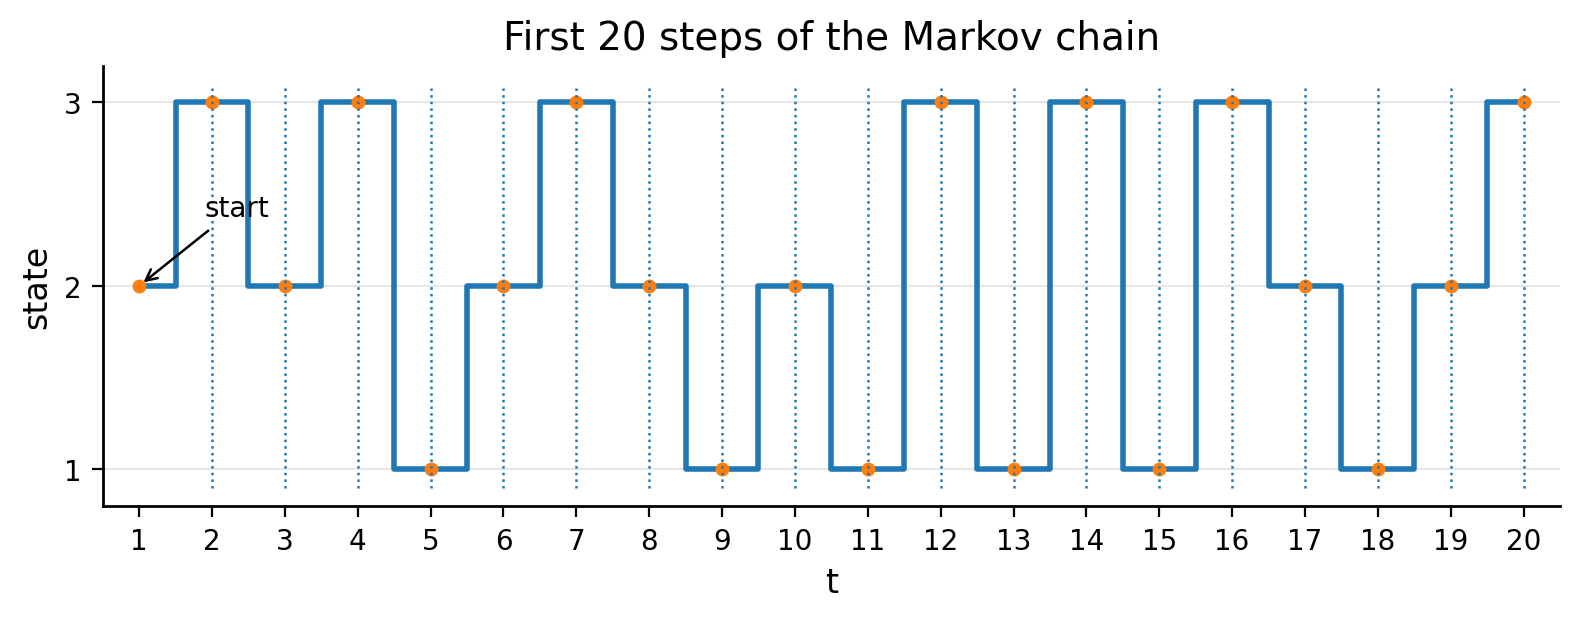
\includegraphics[width=0.85\linewidth]{q2c.png}
                \end{figure}
                
            \end{solution}
            
        \item Find the distribution of the last 100 observations.

            \begin{solution}
    
\begin{lstlisting}[language=python]
import numpy as np

# Assumes x from part (a)
last_100 = x[-100:]
counts = np.bincount(last_100, minlength=4)[1:]  # ignore index 0
proportions = counts / counts.sum()

for s, c, p in zip([1, 2, 3], counts, proportions):
    print(f"State {s}: count = {c:3d}, proportion = {p:.4f}")
\end{lstlisting}

                \begin{table}[h]
                    \centering
                    \begin{tabular}{lcc}
                        \hline
                        \textbf{State} & \textbf{Count} & \textbf{Proportion} \\
                        \hline
                        State 1 & 35 & 0.3500 \\
                        State 2 & 31 & 0.3100 \\
                        State 3 & 34 & 0.3400 \\
                        \hline
                    \end{tabular}
                    \caption{Counts and Proportions for Different States}
                    \label{tab:state_counts_proportions}
                \end{table}

            \end{solution}
            
    \end{enumerate}

\end{document}
